
\selectlanguage{francais}


\chapter{Implémentation et Réalisation}
\label{chap:Chapter 4 title}
\section*{Introduction}

Dans ce chapitre, nous nous présentons les étapes du développement de l'application, en examinant de près les fonctionnalités intégrées ainsi que les ajustements opérés à chaque niveau du système.



\pagebreak

\section{Mise en place de l'environnement de développement}

\hspace{\parindent}Pour commencer le développement de l'application, nous avons initié la configuration de notre environnement de développement en installant une gamme d'outils et de frameworks essentiels tels que Visual Studio, .NET, ABP CLI, entre autres. En parallèle, nous avons également configuré la base de données et établi les connexions nécessaires pour assurer le bon fonctionnement de l'application.

% \begin{figure}[H] 
%     \centering
%     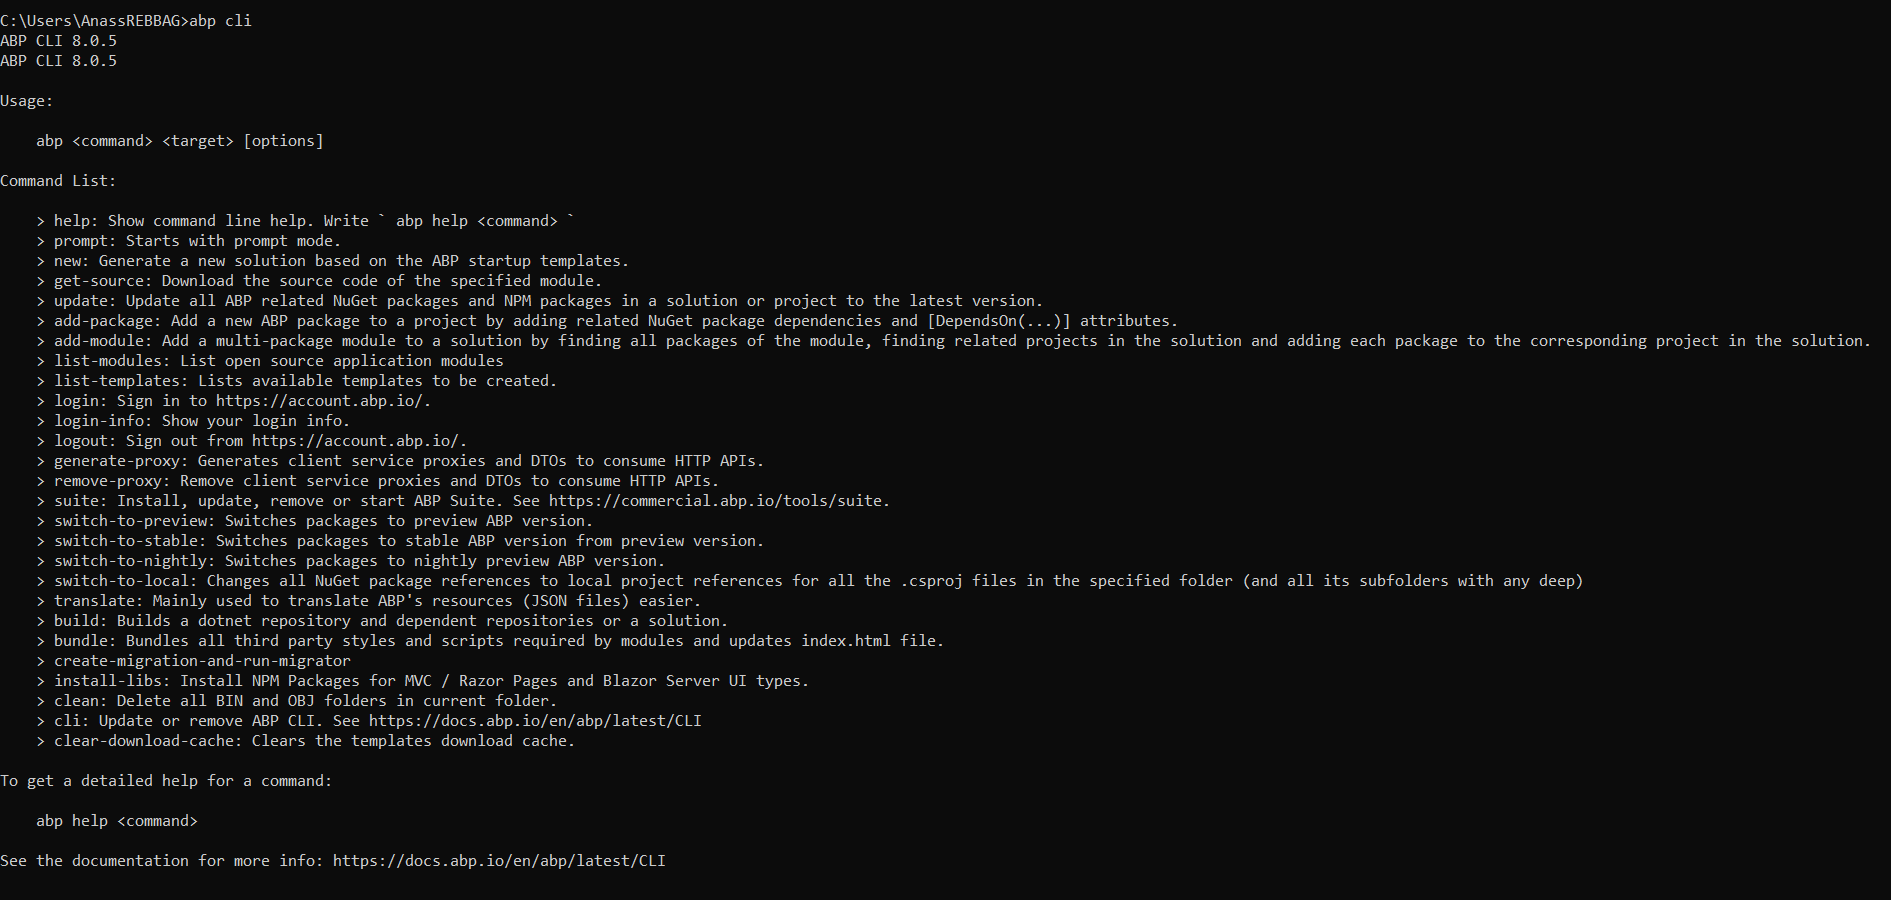
\includegraphics[width=17cm]{Figures/abp cli.PNG}
%         \caption{ABP CLI}
%     %\label{fig:my_label} %Optional (If you want to reference the figure in later chapters)
% \end{figure}

\section{Couche de domaine (Domain Layer)}

Nous avons créé les entités décrites précédemment dans le projet \textbf{B3G.Fawri.CMS.Domain}.


\begin{figure}[H]
    \centering
    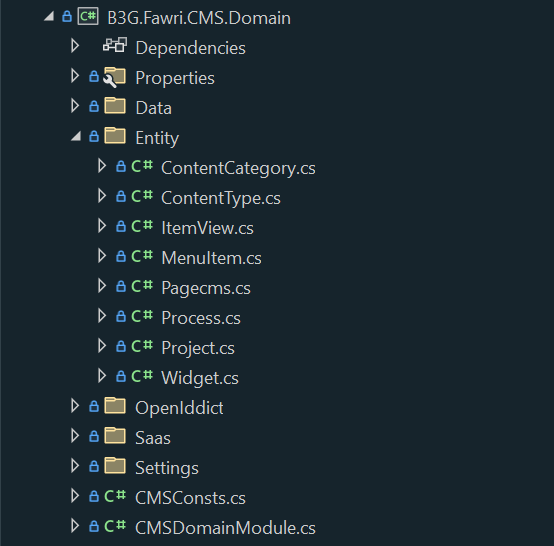
\includegraphics[width=9cm]{Figures/domain folder.PNG}
    \caption{Structure du dossier Domain}
    %\label{fig:my_label} %Optional (If you want to reference the figure in later chapters)
\end{figure}

\section{Couche d'infrastructure (Infrastructure Layer)}

Dans cette couche, nous avons commencé par l'implémentation du contexte de base de données (DbContext) pour Entity Framework. Cette étape se divise en deux parties : la définition des DbSet et la configuration du modèle (builder).

Voici les configurations des builders pour les entités précédemment créées, réalisées dans le projet \textbf{B3G.Fawri.CMS.EntityFrameworkCore}.


\begin{figure}[H]
    \centering
    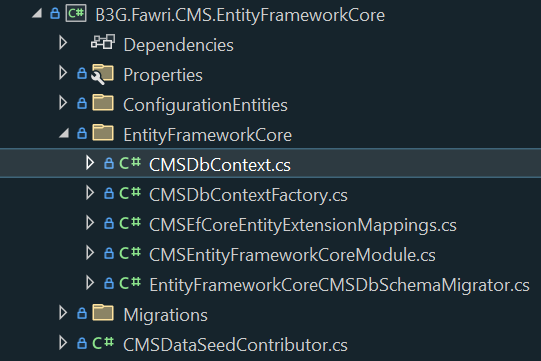
\includegraphics[width=9cm]{Figures/entity fram core folder.PNG}
    \caption{Structure du dossier Infrastructure}
    %\label{fig:my_label} %Optional (If you want to reference the figure in later chapters)
\end{figure}


\begin{figure}[H]
    \centering
    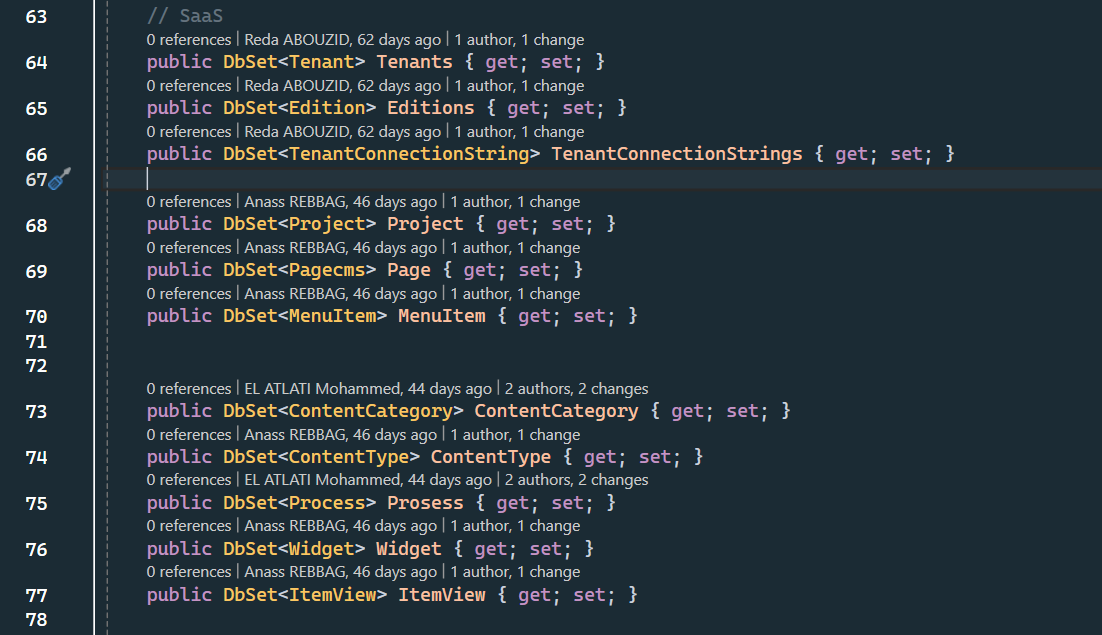
\includegraphics[width=17cm]{Figures/db set code.PNG}
    \caption{Configuration des DbSet}
    %\label{fig:my_label} %Optional (If you want to reference the figure in later chapters)
\end{figure}

\section{Couche d'application (Application Layer)}

Dans cette couche, nous créons les DTOs (Data Transfer Objects) et les interfaces de nos services dans le projet \textbf{B3G.Fawri.CMS.Application.Contracts} . Les DTOs servent de modèles pour transférer les données entre les couches de l'application, facilitant ainsi la communication sans exposer les entités du domaine directement.
\begin{figure}[H]
    \centering
    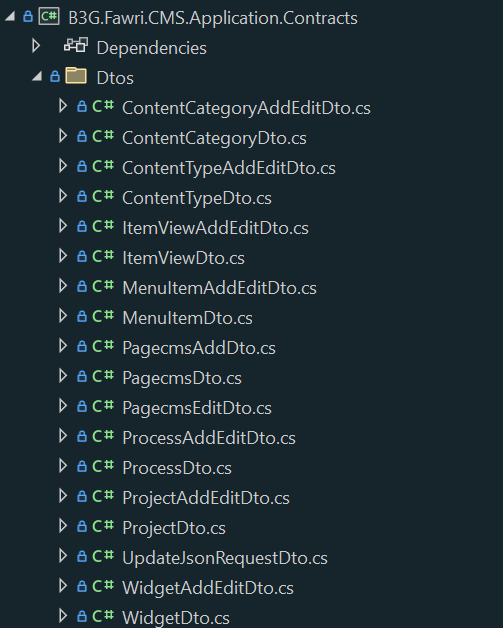
\includegraphics[width=9cm]{Figures/dtos.PNG}
    \caption{Les DTOs dans la couche Application}
    %\label{fig:my_label} %Optional (If you want to reference the figure in later chapters)
\end{figure}

Ensuite, nous procédons à l'implémentation des services dans le projet \textbf{B3G.Fawri.CMS.Application}. Cette étape consiste à définir la logique métier spécifique aux cas d'utilisation de l'application, en respectant les contrats définis par les interfaces précédemment créées. L'implémentation des services inclut la gestion des opérations CRUD (Create, Read, Update, Delete), ainsi que toute autre logique métier nécessaire pour répondre aux exigences fonctionnelles de l'application.

\begin{figure}[H]
    \centering
    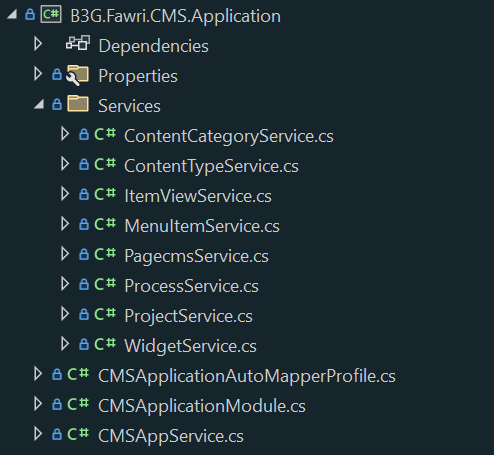
\includegraphics[width=9cm]{Figures/services impl.PNG}
    \caption{Implementation des services}
    %\label{fig:my_label} %Optional (If you want to reference the figure in later chapters)
\end{figure}


Les Webservices implémentés sont :


\begin{table}[H]
    \centering
    \begin{tabular}{|m{5cm}|m{10cm}|}
        \hline
        \textbf{Service} & \textbf{Description}                            \\
        \hline
        CreateProject    & Ce WS permet de créer un projet                 \\
        \hline
        DeleteProject    & Ce WS permet de supprimer un projet             \\
        \hline
        ListProjects     & Ce WS permet de récupérer la liste des projets  \\
        \hline
        GetProjectById   & Ce WS permet de récupérer un projet par son Id. \\
        \hline
        UpdateProject    & Ce WS permet de mettre à jour un projet.        \\
        \hline
    \end{tabular}
    \caption{Les Web services de \textit{Project}}
\end{table}



\begin{table}[H]
    \centering
    \begin{tabular}{|m{5cm}|m{10cm}|}
        \hline
        \textbf{Service} & \textbf{Description}                                         \\
        \hline
        CreatePage       & Ce WS permet de créer une page                               \\
        \hline
        DeletePage       & Ce WS permet de supprimer une page.                          \\
        \hline
        ListPages        & Ce WS permet de récupérer la liste des pages.                \\
        \hline
        GetPageById      & Ce WS permet de récupérer une page par son Id.               \\
        \hline
        UpdatePage       & Ce WS permet de mettre à jour une page.                      \\
        \hline
        UpdatePageJson   & Ce WS permet de mettre à jour une page en utilisant du JSON. \\
        \hline
        GetPagebySlug    & Ce WS permet de récupérer une page par son slug.             \\
        \hline
        GetSlugByPageId  & Ce WS permet de récupérer le slug d'une page par son Id.     \\
        \hline
    \end{tabular}
    \caption{Les Web services de \textit{Page}}
    \label{tab:my_label}
\end{table}





\begin{table}[H]
    \centering
    \begin{tabular}{|m{5cm}|m{10cm}|}
        \hline
        \textbf{Service} & \textbf{Description}                                     \\
        \hline
        CreateMenuItem   & Ce WS permet de créer un élément de menu.                \\
        \hline
        DeleteMenuItem   & Ce WS permet de supprimer un élément de menu.            \\
        \hline
        ListMenuItems    & Ce WS permet de récupérer la liste des éléments de menu. \\
        \hline
        GetMenuItemById  & Ce WS permet de récupérer un élément de menu par son Id. \\
        \hline
        UpdateMenuItem   & Ce WS permet de mettre à jour un élément de menu.        \\
        \hline
    \end{tabular}
    \caption{Les Web services de MenuItem}
    \label{tab:my_label}
\end{table}







\begin{table}[H]
    \centering
    \begin{tabular}{|m{5cm}|m{10cm}|}
        \hline
        \textbf{Service}   & \textbf{Description}                                     \\
        \hline
        CreateContentType  & Ce WS permet de créer un type de contenu.                \\
        \hline
        DeleteContentType  & Ce WS permet de supprimer un type de contenu.            \\
        \hline
        ListContentTypes   & Ce WS permet de récupérer la liste des types de contenu. \\
        \hline
        GetContentTypeById & Ce WS permet de récupérer un type de contenu par son Id. \\
        \hline

        UpdateContentType  & Ce WS permet de mettre à jour un type de contenu         \\
        \hline
    \end{tabular}
    \caption{Les Web services de ContentType}
    \label{tab:my_label}
\end{table}






\begin{table}[H]
    \centering
    \begin{tabular}{|m{5cm}|m{10cm}|}
        \hline
        \textbf{Service}       & \textbf{Description}                                           \\
        \hline
        CreateContentCategory  & Ce WS permet de créer une catégorie de contenu.                \\
        \hline
        DeleteContentCategory  & Ce WS permet de supprimer une catégorie de contenu.            \\
        \hline
        ListContentCategories  & Ce WS permet de récupérer la liste des catégories de contenu   \\
        \hline
        GetContentCategoryById & Ce WS permet de récupérer une catégorie de contenu par son Id. \\
        \hline
        UpdateContentCategory  & Ce WS permet de mettre à jour une catégorie de contenu.        \\
        \hline
    \end{tabular}
    \caption{Les Web services de ContentCategory}
    \label{tab:my_label}
\end{table}




\begin{table}[H]
    \centering
    \begin{tabular}{|m{5cm}|m{10cm}|}
        \hline
        \textbf{Service} & \textbf{Description}                            \\
        \hline
        CreateWidget     & Ce WS permet de créer un widget                 \\
        \hline
        DeleteWidget     & Ce WS permet de supprimer un widget.            \\
        \hline

        ListWidgets      & Ce WS permet de récupérer la liste des widgets. \\
        \hline

        GetWidgetById    & Ce WS permet de récupérer un widget par son Id. \\
        \hline

        UpdateWidget     & Ce WS permet de mettre à jour un widget.        \\

        \hline
    \end{tabular}
    \caption{Les Web services de Widget}
    \label{tab:my_label}
\end{table}














\begin{table}[H]
    \centering
    \begin{tabular}{|m{5cm}|m{10cm}|}
        \hline
        \textbf{Service} & \textbf{Description}                               \\
        \hline
        CreateProcess    & Ce WS permet de créer un processus.                \\
        \hline
        DeleteProcess    & Ce WS permet de supprimer un processus.            \\
        \hline

        ListProcesses    & Ce WS permet de récupérer la liste des processus.  \\
        \hline

        GetProcessById   & Ce WS permet de récupérer un processus par son Id. \\
        \hline

        UpdateProcess    & Ce WS permet de mettre à jour un processus.        \\

        \hline
    \end{tabular}
    \caption{Les Web services de Process}
    \label{tab:my_label}
\end{table}






\begin{table}[H]
    \centering
    \begin{tabular}{|m{5cm}|m{10cm}|}
        \hline
        \textbf{Service} & \textbf{Description}                                    \\
        \hline
        CreateItemView   & Ce WS permet de créer une vue d'élément.                \\
        \hline

        DeleteItemView   & Ce WS permet de supprimer une vue d'élément.            \\
        \hline

        ListItemViews    & Ce WS permet de récupérer la liste des vues d'éléments. \\
        \hline

        GetItemViewById  & Ce WS permet de récupérer une vue d'élément par son Id. \\
        \hline

        UpdateItemView   & Ce WS permet de mettre à jour une vue d'élément.        \\

        \hline
    \end{tabular}
    \caption{Les Web services de ItemView}
    \label{tab:my_label}
\end{table}



Après avoir implémenté les web services, nous démarrons le projet \textbf{B3G.Fawri.CMS.HttpApi.Host}. Cela lance Swagger, qui répertorie et documente tous les web services du système.

La figure suivante représente l’interface Swagger de notre solution :


\begin{figure}[H]
    \centering
    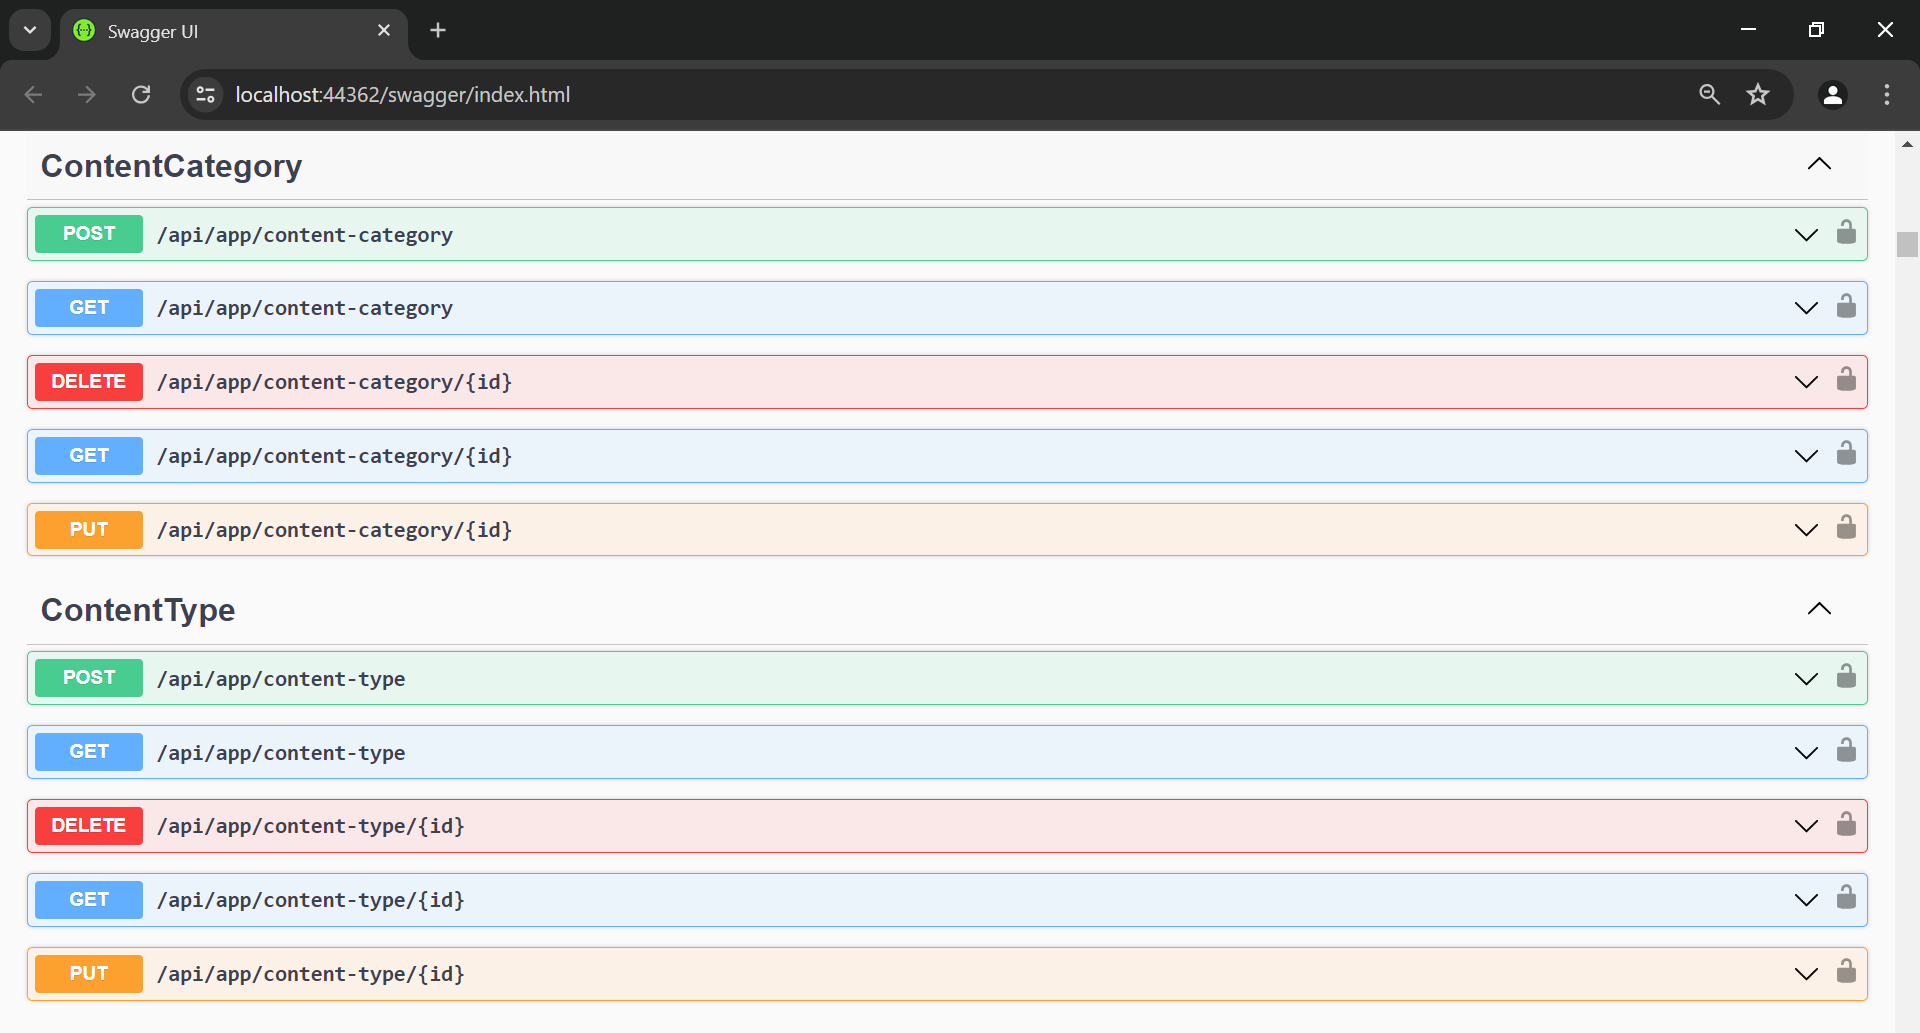
\includegraphics[width=18cm]{Figures/swagger apis.PNG}
    \caption{Interface Swagger}
    %\label{fig:my_label} %Optional (If you want to reference the figure in later chapters)
\end{figure}


\section{Couche de présentation (Presentation Layer)}

\hspace{\parindent}Dans notre projet, la couche de présentation (Presentation Layer) joue un rôle crucial dans l'interaction entre l'utilisateur et l'application. Elle est responsable de l'affichage des informations et de la gestion des interactions utilisateur. Pour Fawri-CMS, le module \textbf{B3G.Fawri.CMS.Web} englobe toutes les interfaces utilisateur et les composants associés. C'est ici que nous créons nos pages (Razor Pages) et que nous gérons l'ensemble des éléments visuels et interactifs de l'application.



\begin{figure}[H]
    \centering
    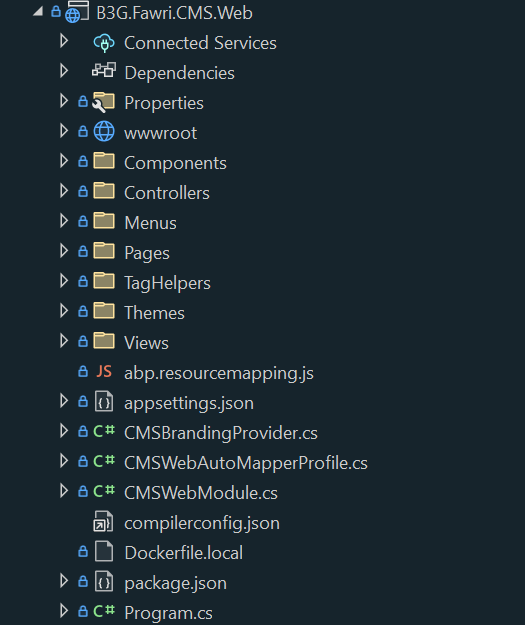
\includegraphics[width=9cm]{Figures/web folder.PNG}
    \caption{Structure du couche Web}
\end{figure}


Cette couche inclut divers dossiers et fichiers essentiels :

\begin{itemize}

    \item \textbf{Components} : Contient les composants réutilisables utilisés dans différentes parties de l'application.

    \item \textbf{Controllers} : Gère les requêtes HTTP et les interactions entre la vue et les modèles.

    \item \textbf{Menus} : Définit la structure de navigation de l'application.

    \item \textbf{Pages} : Contient les Razor Pages, qui sont les vues spécifiques de l'application.

    \item \textbf{TagHelpers} : Fournit des balises personnalisées pour simplifier la création de vues.

    \item \textbf{Themes} : Gère les thèmes et les styles visuels de l'application.

    \item \textbf{Views} : Contient les vues MVC traditionnelles, si nécessaire.

\end{itemize}




\section{Intégration d'Identity Server dans Fawri-CMS avec l'ABP Framework}

\hspace{\parindent}L'intégration d'Identity Server dans Fawri-CMS grâce à l'ABP Framework constitue un élément essentiel pour garantir la sécurité et la gestion efficace de l'identité des utilisateurs. Cette section explore en détail le fonctionnement de cette intégration et ses avantages pour notre application.

L'ABP Framework facilite l'intégration d'Identity Server en fournissant des fonctionnalités prêtes à l'emploi et des outils pour la gestion de l'authentification et de l'autorisation. Voici un aperçu du fonctionnement de cette intégration :

\begin{itemize}
    \item \textbf{Configuration de Identity Server} : L'ABP Framework simplifie la configuration d'Identity Server en fournissant des modèles et des outils pour définir les ressources, les clients et les utilisateurs autorisés à accéder à l'application.

    \item \textbf{Gestion des utilisateurs et des rôles} : Grâce à ASP.NET Core Identity, qui est intégré à l'ABP Framework, la gestion des utilisateurs et des rôles est simplifiée. Identity Server utilise cette infrastructure pour authentifier les utilisateurs et leur attribuer les autorisations appropriées.

    \item \textbf{Authentification basée sur les standards ouverts} : Identity Server prend en charge les protocoles d'authentification standard tels que OAuth 2.0 et OpenID Connect, assurant ainsi une authentification sécurisée et compatible avec les normes industrielles.

    \item \textbf{Centralisation de l'authentification et de l'autorisation} : En intégrant Identity Server, Fawri-CMS bénéficie d'une solution centralisée pour gérer l'authentification et l'autorisation des utilisateurs, ce qui simplifie le développement et la maintenance de l'application.
\end{itemize}

Dans notre cas, nous avons choisi de séparer le serveur d'authentification en un projet distinct (\textbf{B3G.Fawri.CMS.AuthServer}) afin de pouvoir le personnaliser au fur et à mesure de l'avancement de ce projet.


\begin{figure}[H]
    \centering
    
\includegraphics[width=9cm]{Figures/login ui.PNG}
    \caption{Interface de l'authentification}
\end{figure}


\section{Gestion des tenants}

\hspace{\parindent}Dans notre solution Fawri-CMS, la gestion des tenants (ou multi-tenance) est un aspect crucial qui permet de servir efficacement plusieurs clients avec une seule instance de l'application. Grâce à l'ABP Framework, nous avons mis en place une architecture multi-tenant robuste qui offre isolation, personnalisation et sécurité pour chaque tenant.

Dans notre projet Fawri-CMS, nous avons implémenté la gestion des tenants en utilisant l'interface IMultiTenant fournie par l'ABP Framework. Chaque entité de notre application inclut un identifiant de tenant (TenantId), garantissant ainsi une isolation et une personnalisation des données pour chaque client (tenant).


\begin{figure}[H]
    \centering
    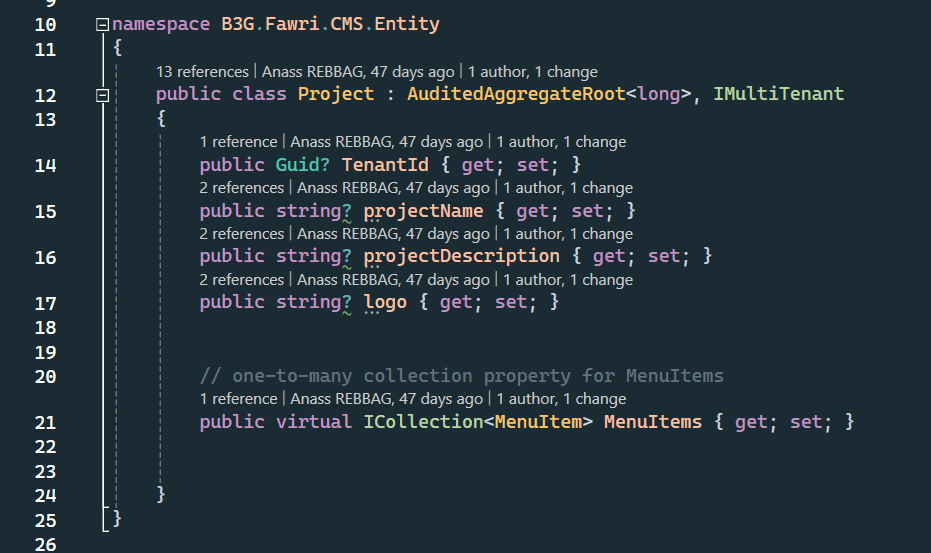
\includegraphics[width=13cm]{Figures/tenant code.PNG}
    \caption{Implementation de la \textit{multitenancy}}
\end{figure}

% \section{Gestion des permissions}

% \hspace{\parindent}La gestion des permissions représente un pilier fondamental garantissant la sécurité et le contrôle d'accès à diverses fonctionnalités et ressources de notre application. Cette fonctionnalité permet de définir les droits d'accès des utilisateurs en fonction de leur rôle et de leurs responsabilités au sein de l'organisation, assurant ainsi une répartition adéquate des privilèges. Grâce à cette approche, les administrateurs disposent d'un contrôle précis sur les actions pouvant être effectuées par chaque utilisateur dans l'application.

% Par ailleurs, ABP Framework enrichit notre projet en mettant à disposition un module spécifique dédié à la gestion des permissions. Cette intégration harmonieuse offre une solution complète pour la définition et la gestion des autorisations. Le module permet une granularité fine dans la définition des permissions, permettant de spécifier des autorisations pour chaque action et ressource de l'application. De plus, il offre la souplesse nécessaire pour activer ou désactiver ces permissions en fonction des rôles, des utilisateurs ou des clients. Ainsi, notre équipe peut contrôler avec précision les actions autorisées pour chaque utilisateur, garantissant une gestion sécurisée et efficace des autorisations au sein de notre système.

\section{Interface d’utilisateur}

\subsection{Authentification de l’application :}

\hspace{\parindent}Lorsqu'un utilisateur, tel que le super administrateur (personnel de B3G) ou l'administrateur d'un tenant, souhaite accéder à la plateforme Fawri-CMS, le système lui demande de s'authentifier en fonction de son profil. La figure ci-dessous illustre la page de connexion.


\begin{figure}[H]
    \centering
    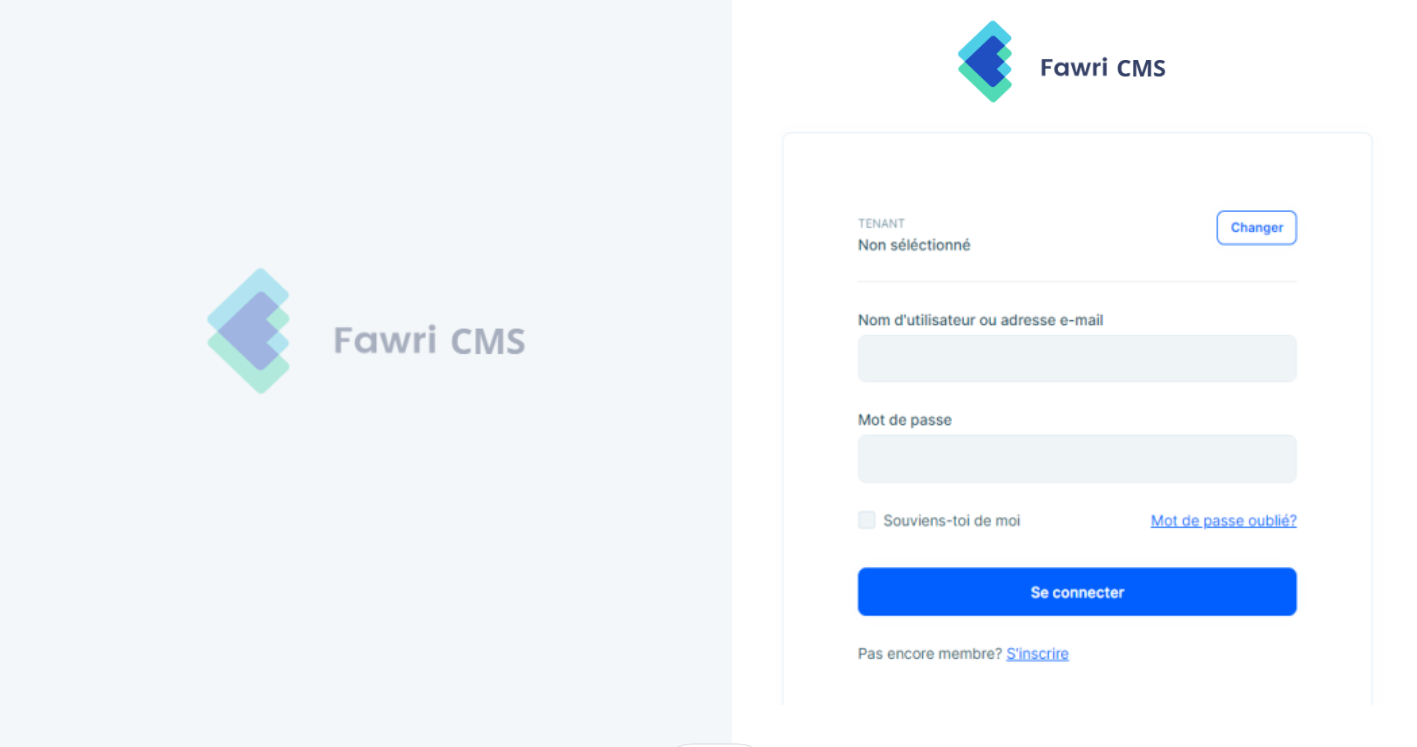
\includegraphics[width=18cm]{Figures/full loging page.PNG}
    \caption{Page de l'authentification}
\end{figure}


\subsection{Interface Super Admin}

\hspace{\parindent}Le Super Admin est le pilier central de l'administration de Fawri-CMS. Il agit en tant que gardien principal de la plateforme, responsable de sa configuration initiale, de son bon fonctionnement quotidien et de son évolution continue. En tant que point focal, le Super Admin détient un ensemble de privilèges et de responsabilités étendus qui lui permettent de superviser tous les aspects de l'application.

Dans cette partie, nous allons présenter les fonctionnalités que seul le Super Admin peut effectuer, telles que la création d'éditions et de tenants. Le schéma suivant représente l'acheminement que nous allons suivre pour présenter les interfaces du Super Admin.

\begin{figure}[H]
    \centering
    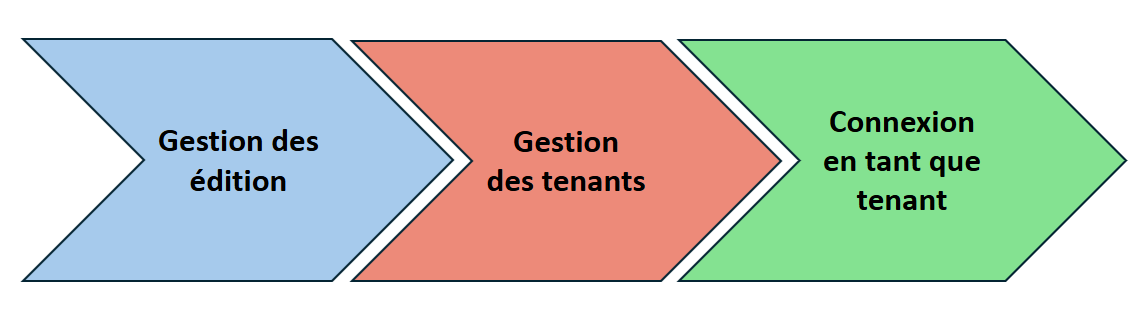
\includegraphics[width=11cm]{Figures/fonctionnalite super admin.PNG}
    \caption{Les fonctionnalités du super admin}
\end{figure}

\begin{enumerate}
    \item \textbf{Gestion des Éditions} :
          Dans Fawri-CMS, la gestion des éditions est une fonctionnalité essentielle qui permet au Super Admin de configurer et de personnaliser les offres pour différents segments de clients. Les éditions permettent de définir des niveaux de service distincts, chacun avec ses propres fonctionnalités et configurations spécifiques.

          Le Super Admin a la responsabilité de créer, modifier et gérer les éditions. Ces éditions définissent les différentes versions de l'application qui peuvent être proposées à divers groupes de clients (tenants).

          \begin{figure}[H]
              \centering
              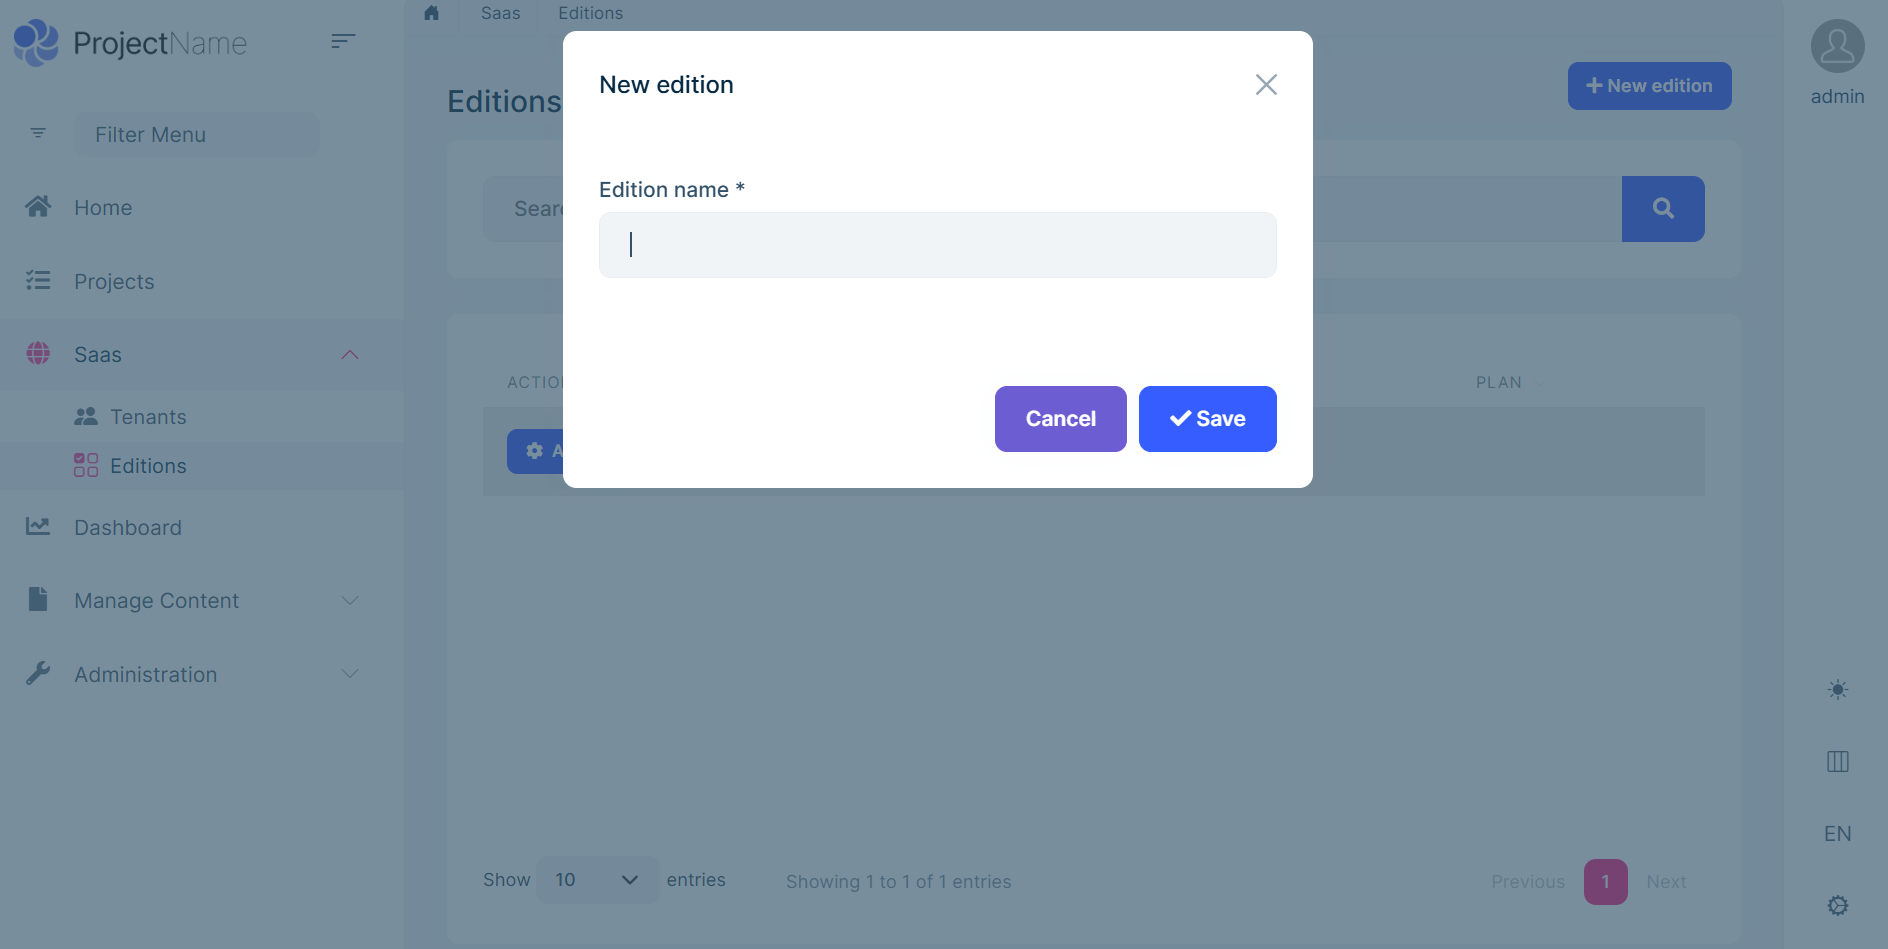
\includegraphics[width=17cm]{Figures/new edition.PNG}
              \caption{Interface d'ajout d'une édition}
          \end{figure}

    \item \textbf{Gestion des tenants} :

          \begin{figure}[H]
              \centering
              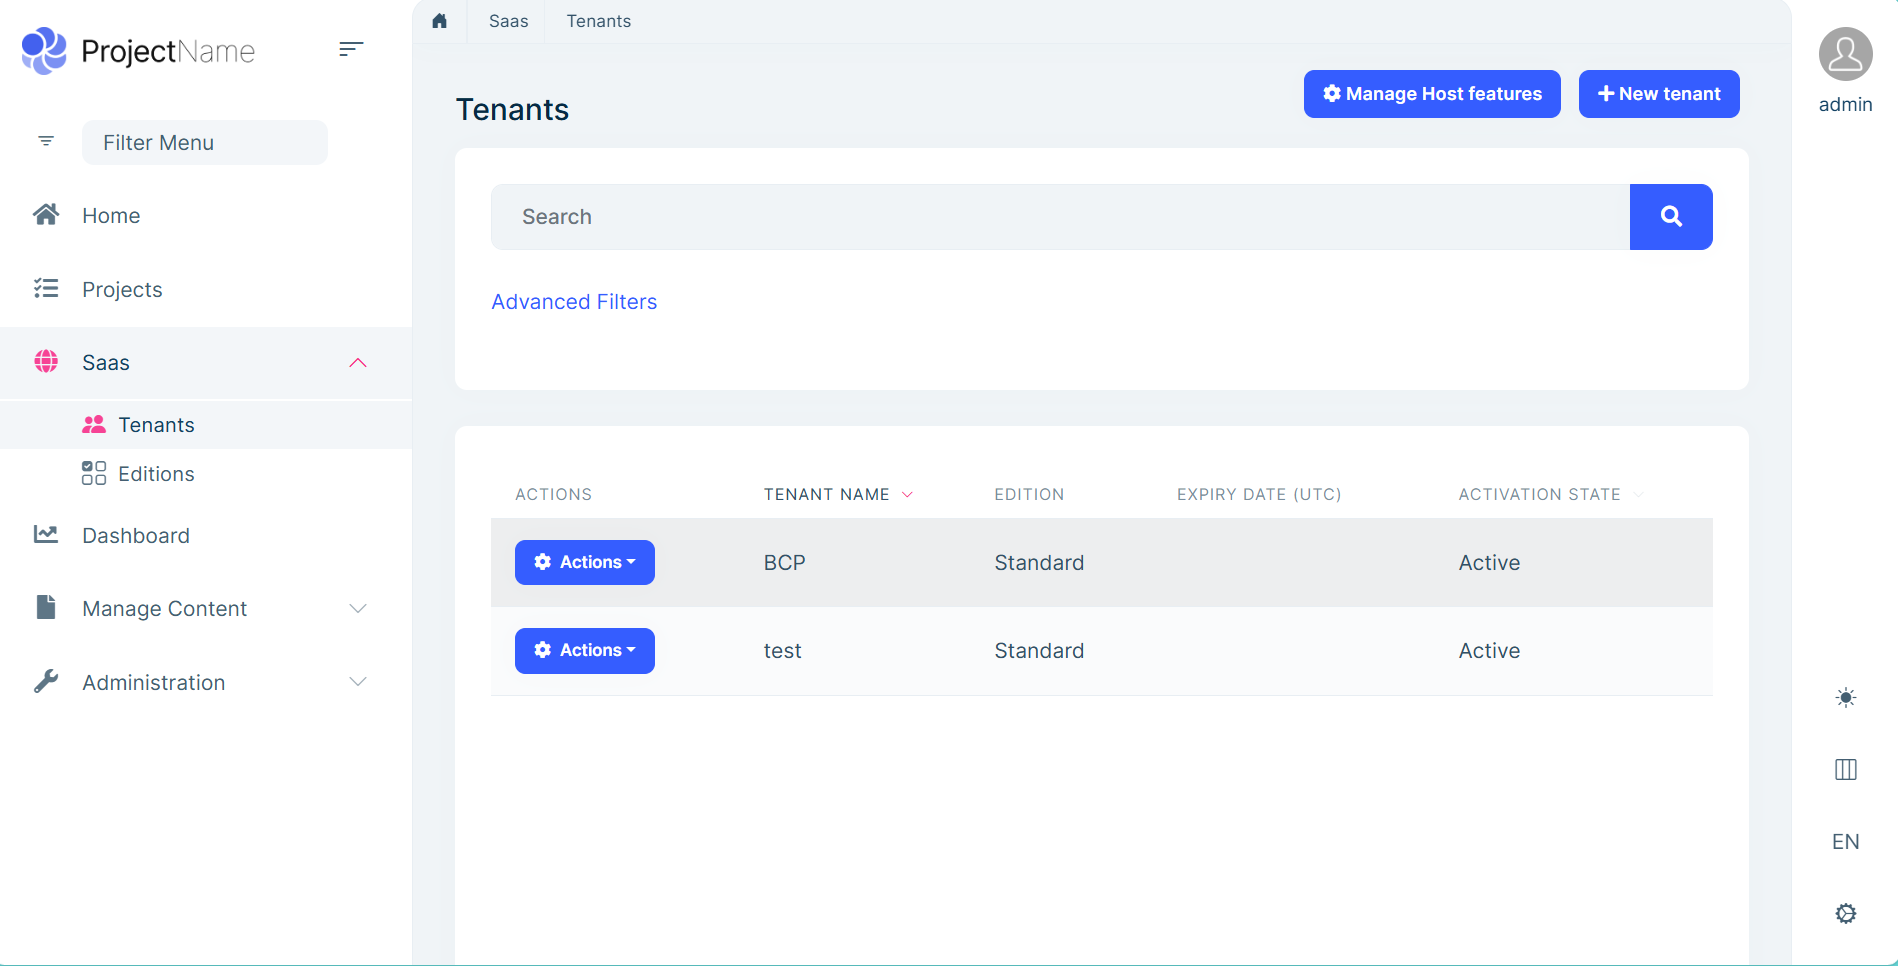
\includegraphics[width=17cm]{Figures/tenant screenshot.PNG}
              \caption{Liste des tenants}
          \end{figure}

          \hspace{\parindent}Dans notre solution Fawri-CMS, le Super Admin a la possibilité de configurer la chaîne de connexion pour chaque nouveau tenant lors de sa création. Cette flexibilité permet de personnaliser la base de données utilisée par chaque tenant, garantissant une isolation appropriée des données et une gestion efficace des ressources. Le Super Admin peut également choisir d'utiliser la chaîne de connexion par défaut pour les nouveaux tenants si aucune personnalisation spécifique n'est nécessaire.



    \item \textbf{Connexion en tant que tenant} :

          Étant donné que le Super Admin a un contrôle total de l'application, il peut se connecter en tant que tenant. De plus, il a accès à toutes les fonctionnalités de l'application.




\end{enumerate}


\subsection{Interface Tenant}

Dans cette partie, nous allons présenter les fonctionnalités spécifiques au Tenant Admin. Ces fonctionnalités incluent la gestion des projets, la gestion de contenu, la gestion des utilisateurs et des permissions au sein de leur propre espace de travail (tenant). Le Tenant Admin joue un rôle crucial en administrant et en personnalisant les paramètres et les ressources disponibles pour les utilisateurs finaux dans leur tenant.



% \begin{figure}[H] 
%     \centering
%     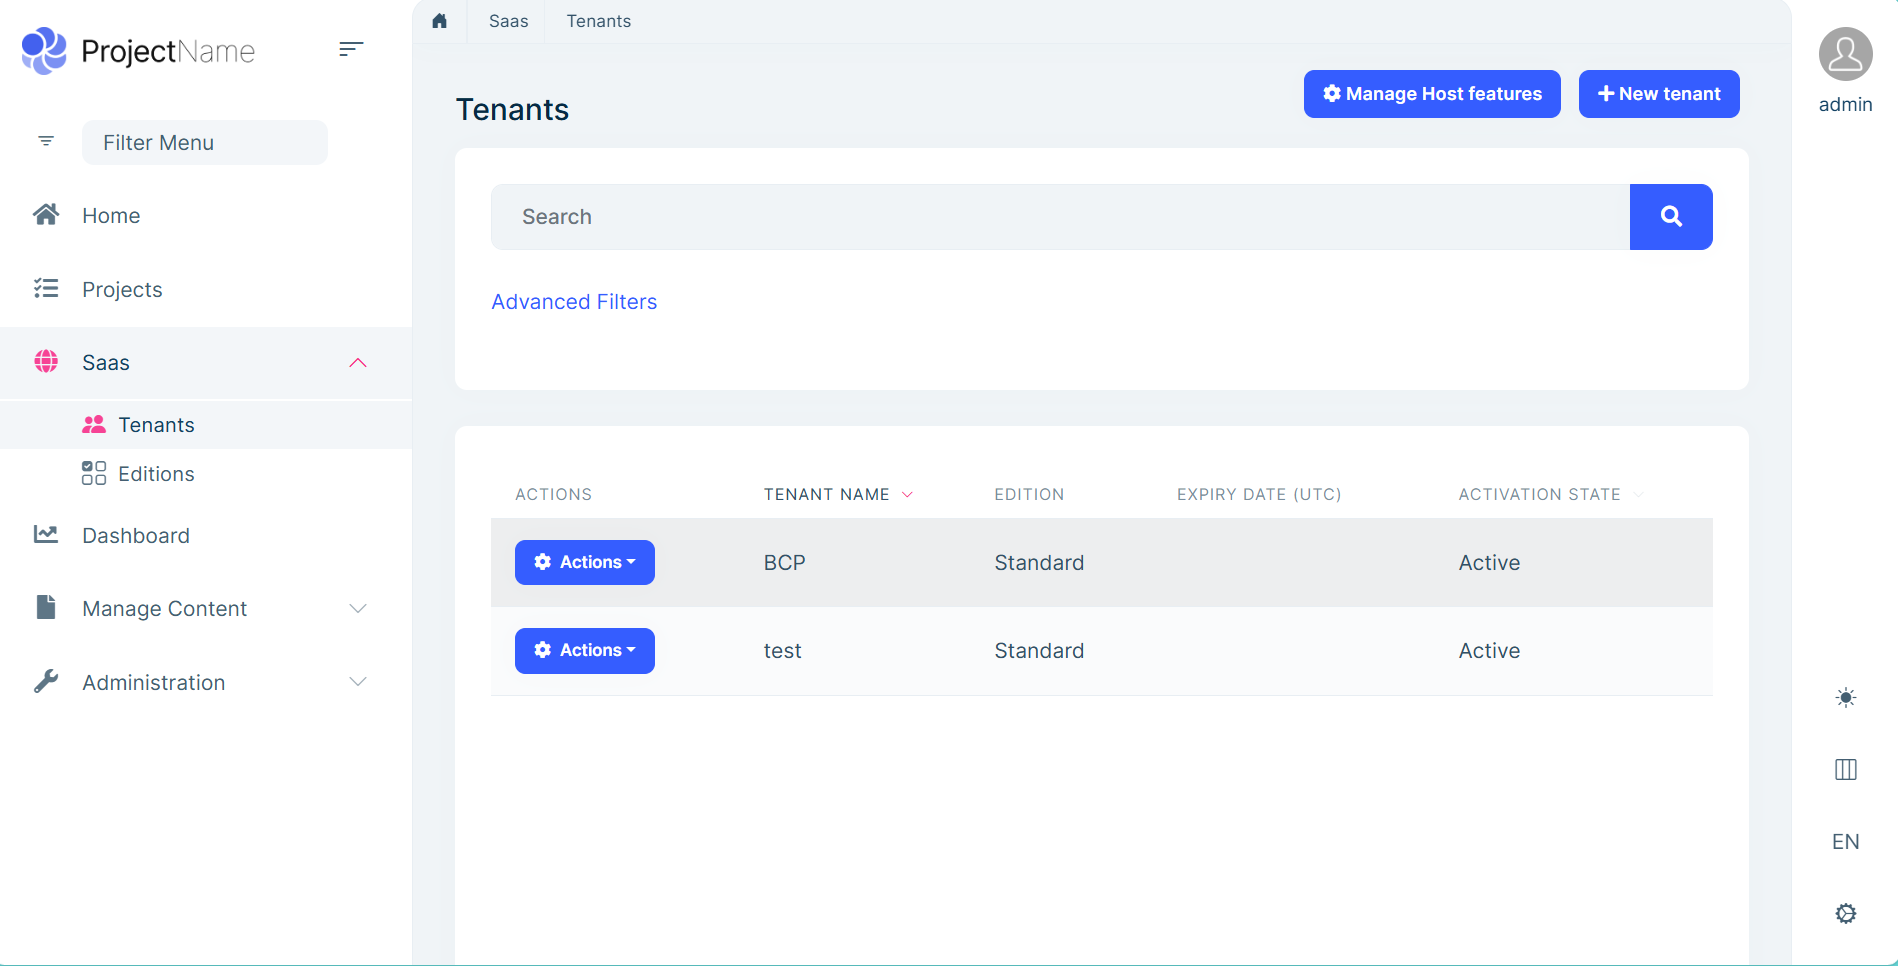
\includegraphics[width=17cm]{Figures/tenant screenshot.PNG}
%     \caption{Interface de l'authentification}
% \end{figure}

\begin{enumerate}
    \item \textbf{Création d’un nouveau projet} :



          \begin{figure}[H]
              \centering
              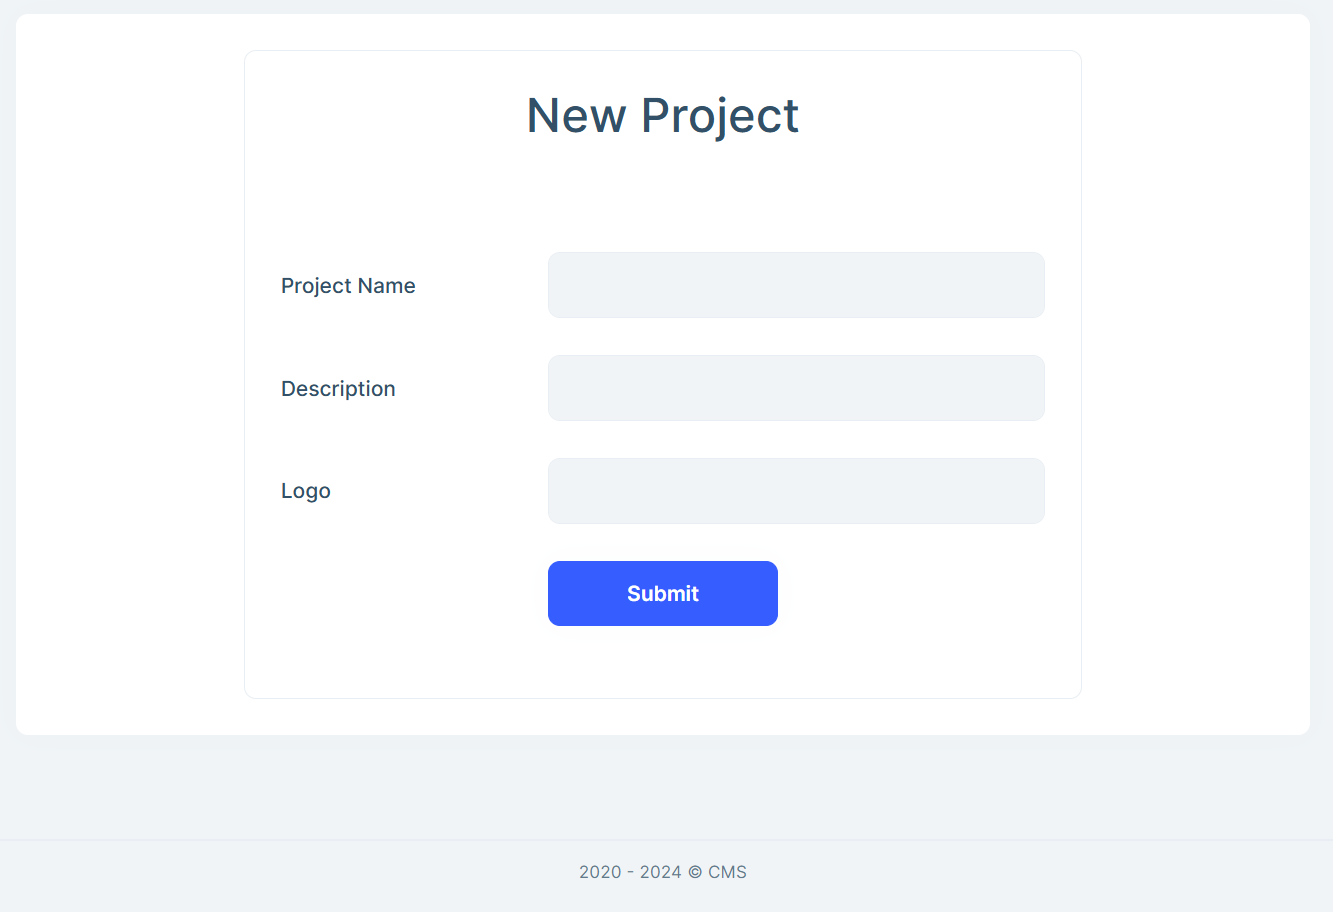
\includegraphics[width=10cm]{Figures/new project.PNG}
              \caption{Création d'un nouveau projet}
          \end{figure}

          \begin{figure}[H]
              \centering
              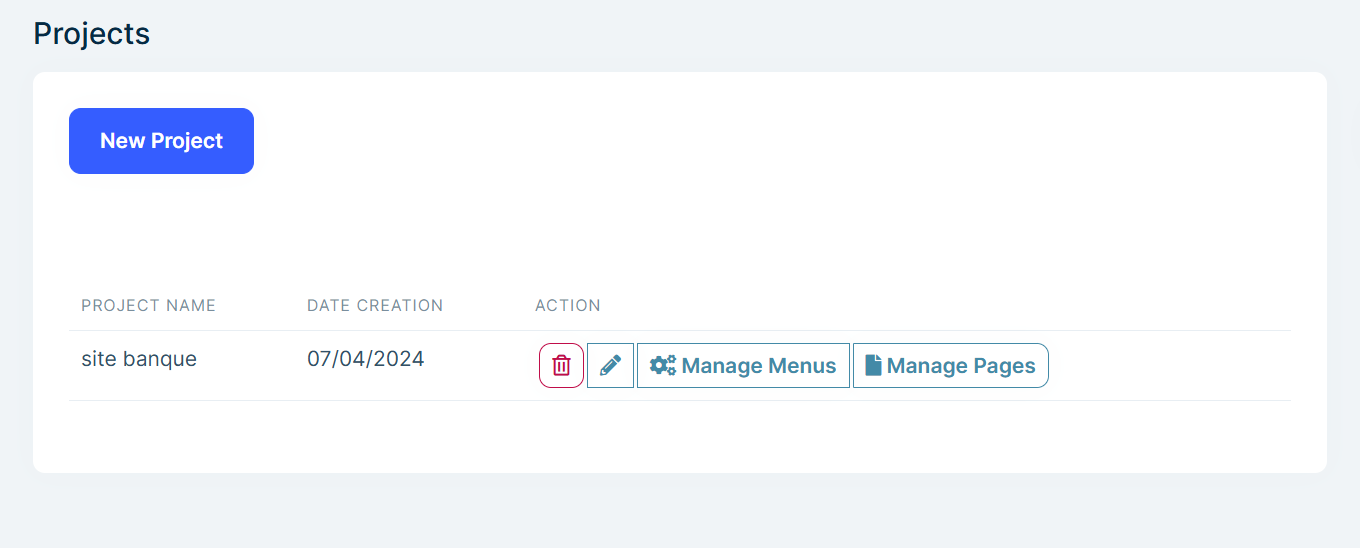
\includegraphics[width=17cm]{Figures/list projects.PNG}
              \caption{Consultation des projets}
          \end{figure}



    \item \textbf{Gestion des pages} :

          \begin{figure}[H]
              \centering
              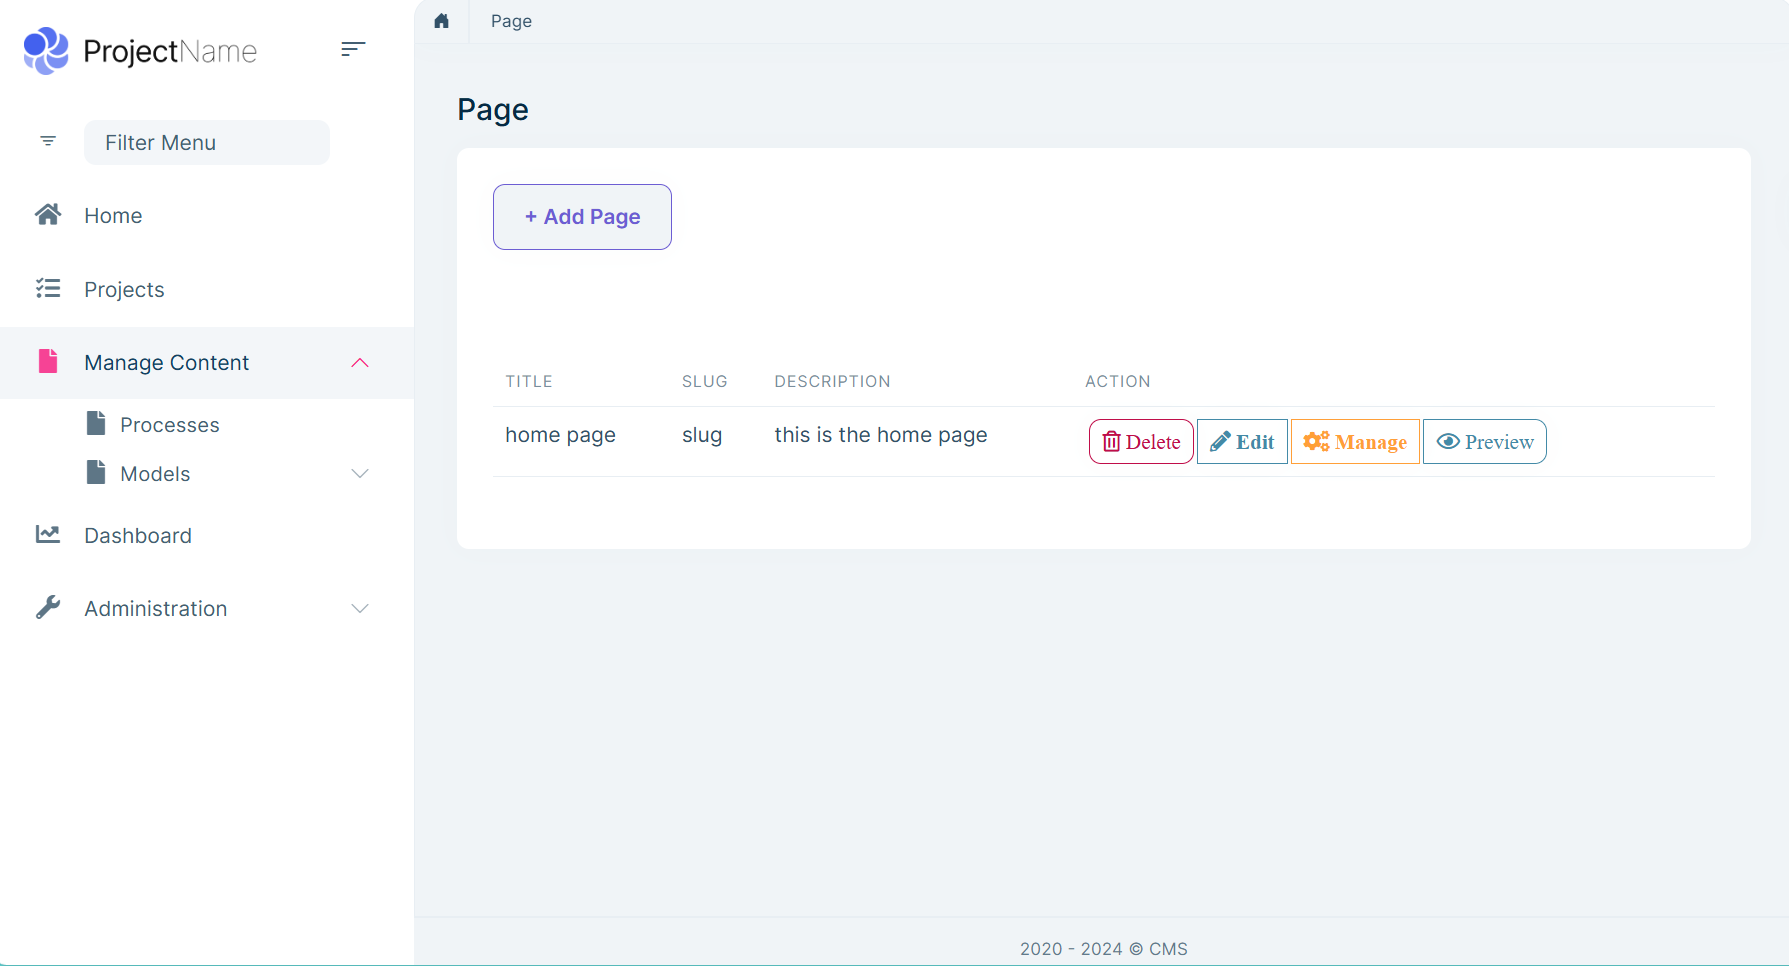
\includegraphics[width=17cm]{Figures/list pages.PNG}
              \caption{Consultation des pages}
          \end{figure}


          \begin{figure}[H]
              \centering
              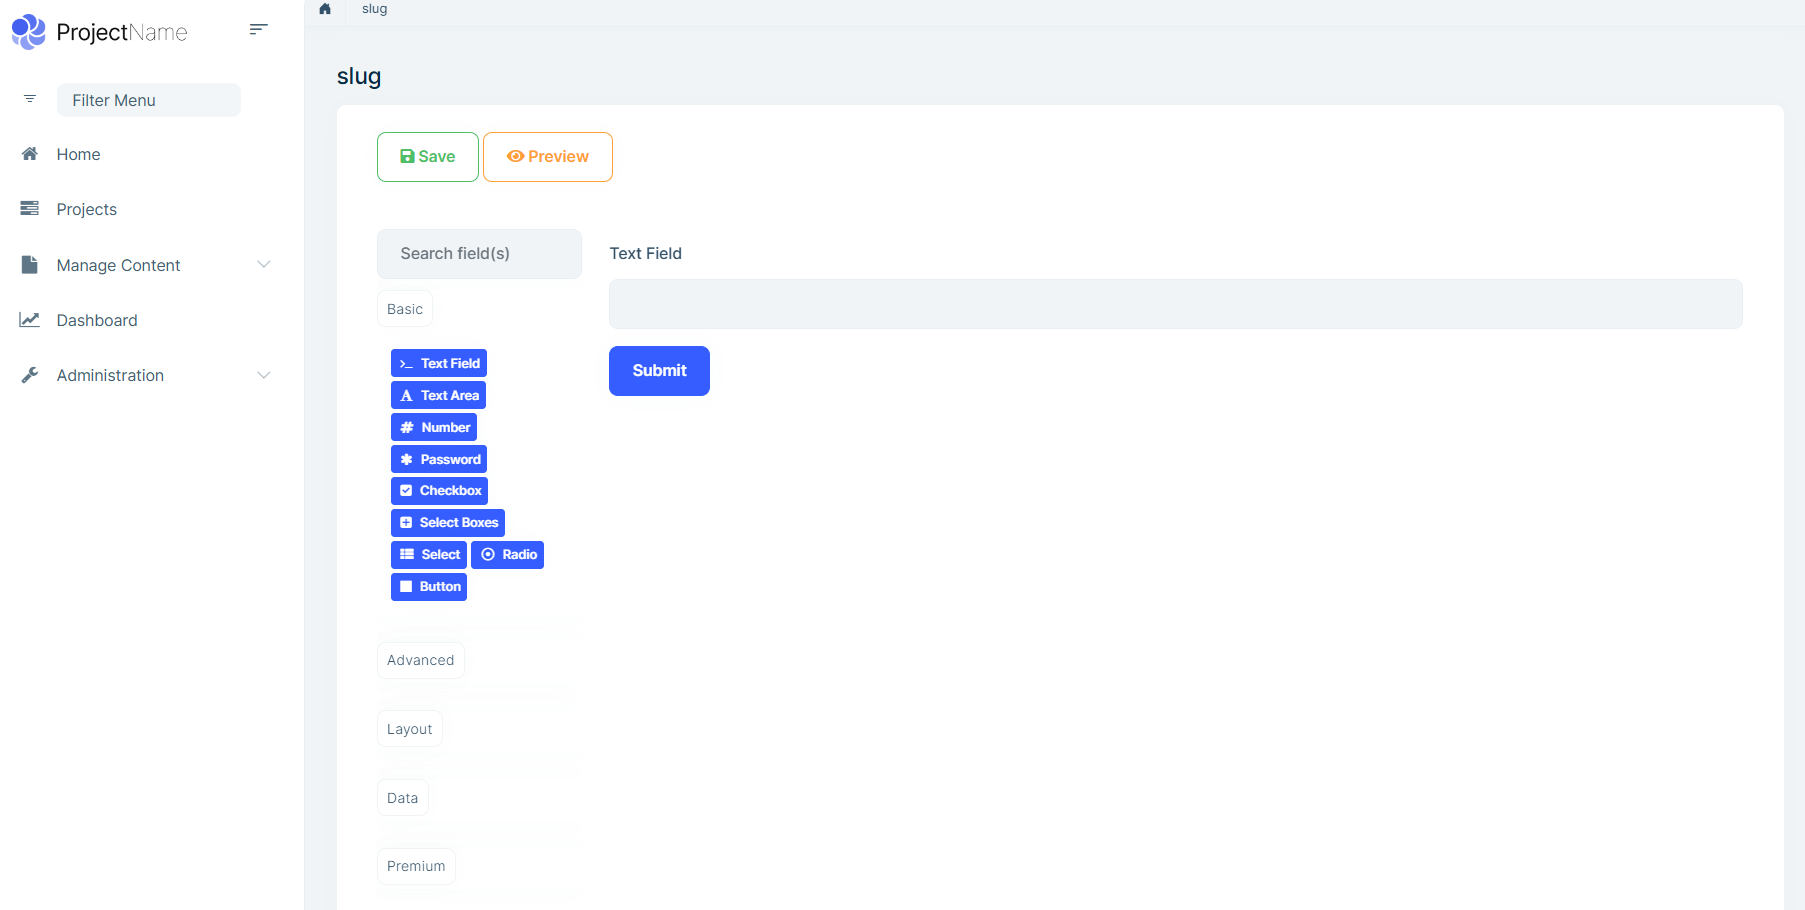
\includegraphics[width=17cm]{Figures/manage page.PNG}
              \caption{Gestion des pages}
          \end{figure}


          En plus des composants de base de cet éditeur basé sur Form.io, nous avons ajouté un nouveau composant "Process" dans la section Premium (voir figure suivante). Ce composant nous permet d'utiliser les processus créés avec Fawri-Flow, favorisant ainsi la réutilisation des composants et des processus existants au lieu de les développer à partir de zéro. Ce composant "Process" récupère la liste des processus créés avec Fawri-Flow et nous permet de les intégrer facilement à nos pages.



          \begin{figure}[H]
              \centering
              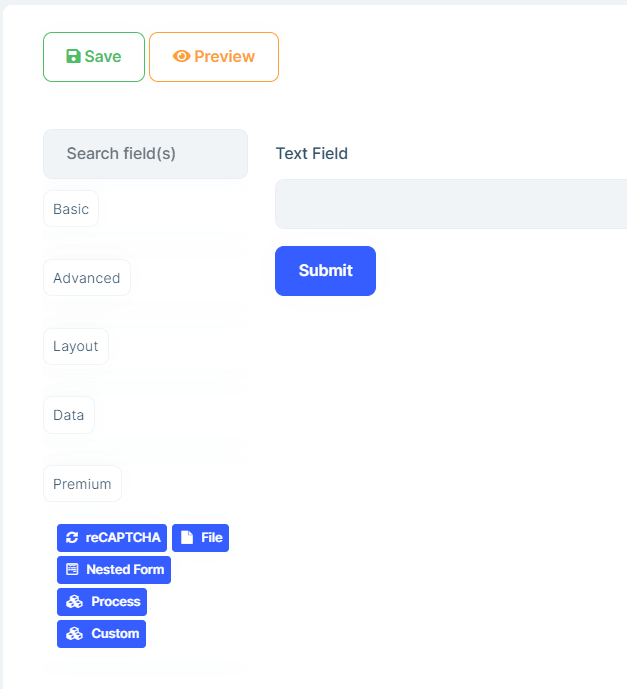
\includegraphics[width=9cm]{Figures/process 1.PNG}
              \caption{Organisation des Processus}
          \end{figure}
          \begin{figure}[H]
              \centering
              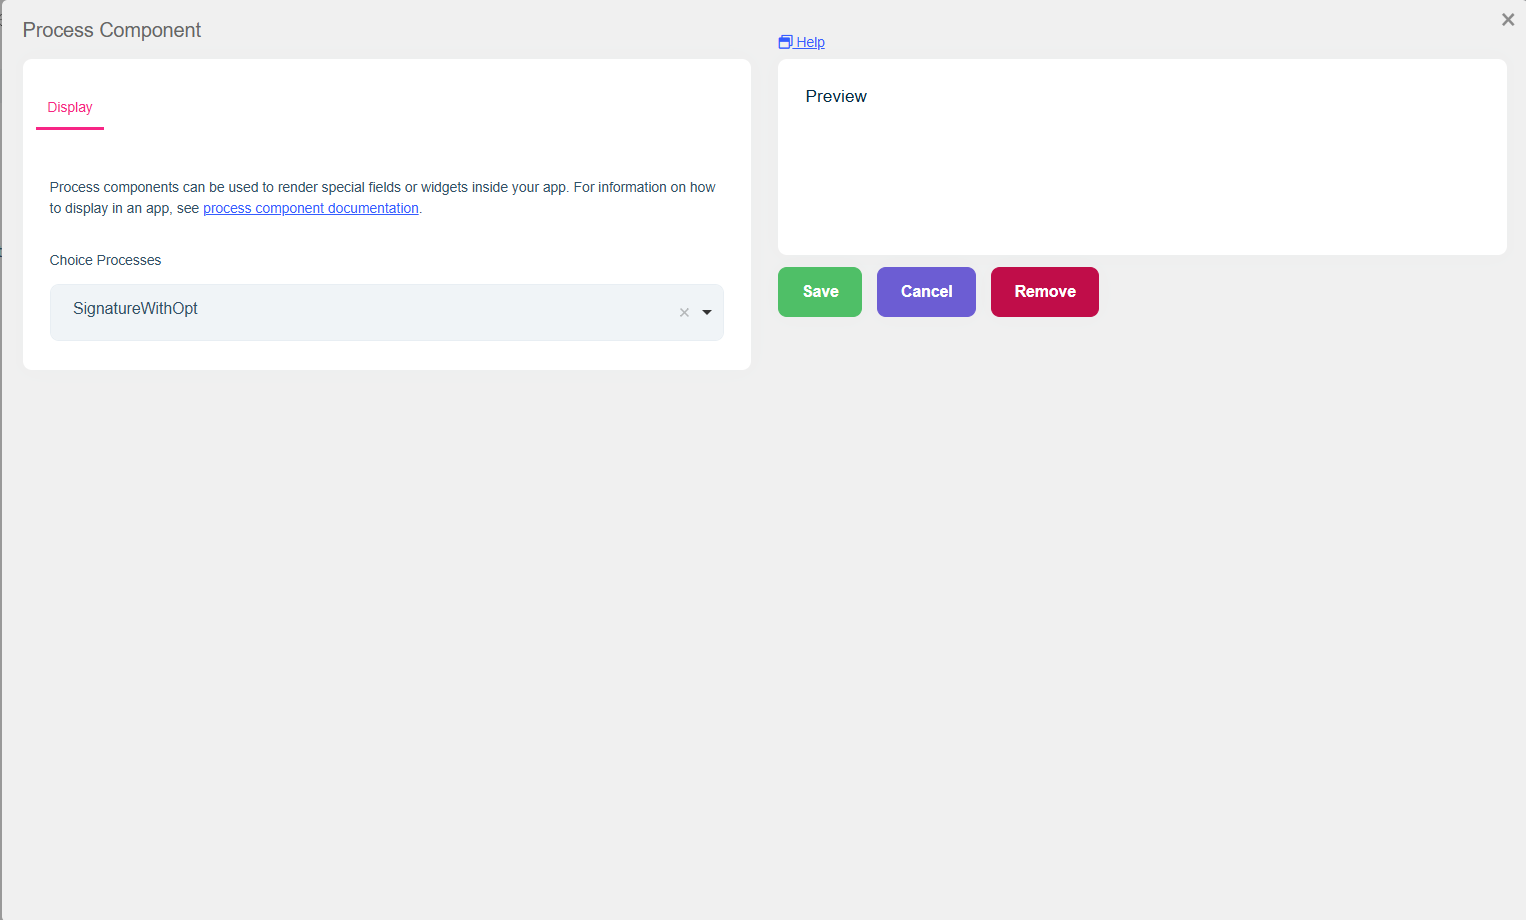
\includegraphics[width=17cm]{Figures/process 2.PNG}
              \caption{Ajout du processus \textit{SignatureWithOtp}}
          \end{figure}

          Le processus sélectionné est ajouté à la page. Dans notre cas, nous avons choisi le processus du service vérification avec OTP comme exemple.

          Après la création de notre page, on clique sur "Save" pour sauvegarder la page créée (sauvegarder le JSON généré) et on visualise la page en cliquant sur "Preview".


    \item \textbf{La gestion des menus} :
          Après la création et l'édition des pages, nous passons à la création des éléments de menu. Cela se fait en attribuant les éléments de menu soit à une page créée dans notre projet, soit à une URL externe.

          \begin{figure}[H]
              \centering
              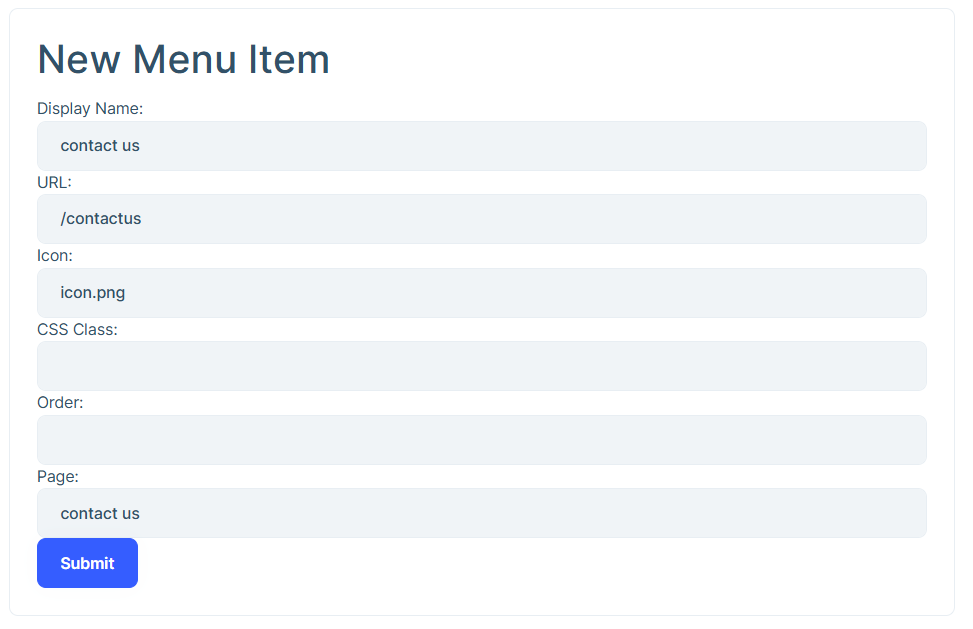
\includegraphics[width=12cm]{Figures/menu item.PNG}
              \caption{L'ajout d'un élément au menu}
          \end{figure}

          Lors de la création d'un élément de menu dans notre projet Fawri-CMS, nous avons la possibilité de l'affecter à une page spécifique que nous avons créée, ou de le lier à une URL externe. De plus, il est possible de créer des sous-menus pour structurer le contenu de manière hiérarchique. Cette flexibilité permet une personnalisation et une organisation optimale de la navigation au sein de l'application, améliorant ainsi l'expérience utilisateur.




    \item \textbf{La gestion des permissions} :


          La gestion des permissions, qui consiste à définir les droits d'accès à différents niveaux, est essentielle dans tout système. Elle implique notamment la mise en place de rôles tels que le super administrateur, qui détient des privilèges étendus sur l'ensemble du système, et l'administrateur du locataire (Tenant Admin), chargé de gérer les autorisations au niveau spécifique du locataire.

          \begin{figure}[H]
              \centering
              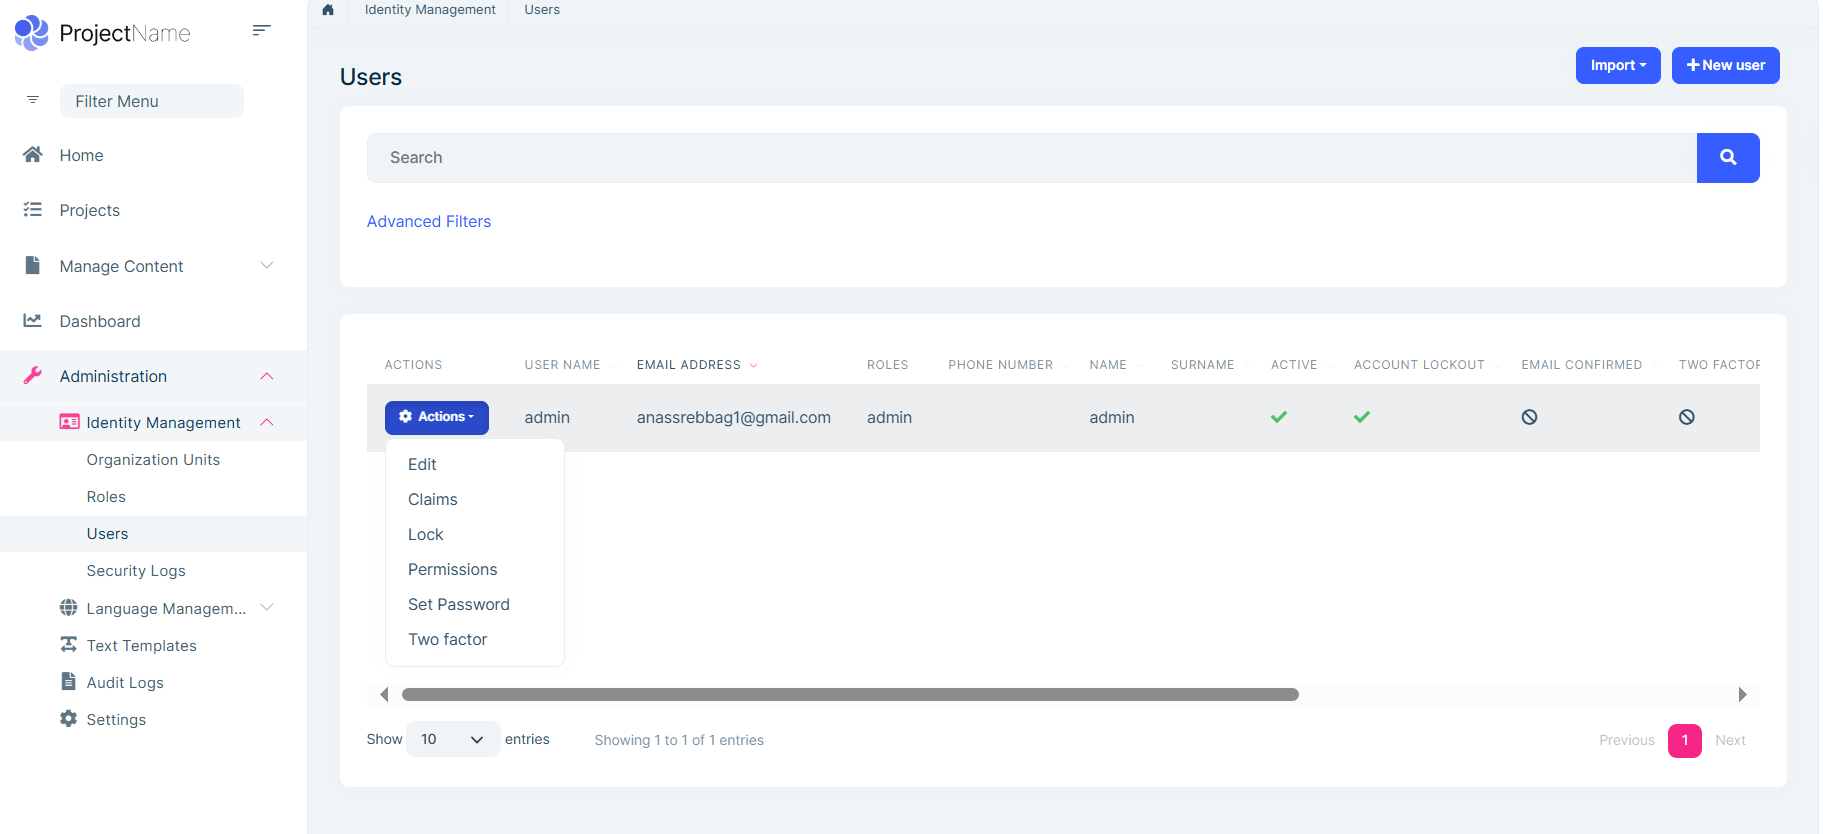
\includegraphics[width=17cm]{Figures/permission.PNG}
              \caption{Gestion des permissions}
          \end{figure}





\end{enumerate}



















\newpage

\section*{Conclusion}

\hspace{\parindent}Le chapitre portant sur l'Implémentation et la Réalisation a constitué une étape fondamentale de notre projet, marquant son passage de l’analyse et la conception à la mise en œuvre opérationnelle. Nous avons commencé par établir un environnement de développement adéquat, puis avons exploré en profondeur les différentes couches de l'architecture logicielle, assurant ainsi une base solide pour notre application. L'intégration d'Identity Server dans Fawri-CMS grâce à l'ABP Framework a permis de garantir la sécurité et la gestion efficace de l'authentification des utilisateurs. De plus, la mise en place de la gestion des tenants et des permissions a offert une flexibilité et une adaptabilité indispensables à notre système. À travers le développement d'une interface utilisateur intuitive pour les Super Admins et les Tenants, nous avons veillé à ce que l'expérience utilisateur soit optimale et conviviale. En somme, ce chapitre a été crucial pour matérialiser notre projet, en fournissant les bases techniques et fonctionnelles nécessaires à son succès et à sa pérennité.

\pagebreak